% !TEX root = main.tex

\subsection{上板}
\qquad 使用Basys3板运行所设计的CPU时,需要通过4个七段数码管来查看当前CPU的执行情况。
\par 只考虑指令和数据的低8位,即指令存储器中的指令地址范围和数据存储器中的数据地址范围均为 \verb'0x00'$\sim$ \verb'0xFF'。
\par 通过Basys3板上的开关SW15、SW14选择七段数码管显示的内容,具体显示的功能码如表\ref{tab:seg_code}所示。
% Table generated by Excel2LaTeX from sheet 'Display'
\begin{table}[htbp]
  \centering\wuhao
  \caption{数码管显示功能码}
    \begin{tabular}{|r|r|l|l|}
    \hline
    \multicolumn{1}{|c|}{SW15} & \multicolumn{1}{c|}{SW14} & \multicolumn{1}{c|}{左边} & \multicolumn{1}{c|}{右边} \bigstrut\\
    \hline
    0     & 0     & 当前PC  & 下条PC \bigstrut\\
    \hline
    0     & 1     & rs寄存器地址 & rs寄存器数据 \bigstrut\\
    \hline
    1     & 0     & rt寄存器地址 & rt寄存器数据 \bigstrut\\
    \hline
    1     & 1     & ALU结果输出 & DB总线数据 \bigstrut\\
    \hline
    \end{tabular}%
  \label{tab:seg_code}%
\end{table}%

\subsection{七段数码管显示电路}
\qquad基本实现步骤如下:
\begin{enumerate}
    \item 对Basys3板系统时钟信号(100MHz)进行分频,使得数码管内容能够正常显示。频率不宜过快,过快会导致全部数码管显示的都是8;也不宜过慢,否则数码管会出现暂留现象,无法连续显示。在本次实现中采用10kHz的频率进行显示。
    \item 用上面得到的频率生成4进制计数器,用于产生4个数位选信号AN3-AN0。这4个数可控制哪个数码管亮,一共四组编码(1110、1101、1011、0111),每组编码中只有一位为0(亮),其余都为1(灭),在每一个位选信号到来之时更新数码管显示。其实前两步可以一并完成,见第\ref{sec:appendix}章分频计数器一节。
    \item 将从CPU接收到的相应数据转换为数码管显示信号,与位选信号一起送往数码管显示输出。
\end{enumerate}

\subsection{其他注意事项}
\begin{enumerate}
    \item 共阳极数码管\\
    Basys3板的数码管均为共阳极,故设置七段数码管和位选信号时都要考虑0为亮,1为灭。
    \item 两个时钟信号\\%https://stackoverflow.com/questions/29737369/place-30-574-poor-placement-for-routing-between-an-io-pin-and-bufg
    CPU工作时钟和Basys3板系统时钟是两个不同的时钟,但是FPGA只支持单一全局时钟,否则在routing阶段会报错
    \begin{center}\verb'Poor placement for routing between an IO pin and BUFG'\end{center}
    故需要采取其他方法。只设置全局时钟为\verb'clk',并将CPU工作时钟\verb'clk_cpu'与其同步,即在每一个\verb'clk'上升沿时,赋值\verb'in<=clk_cpu',通过下面消抖处理后,将\verb'in'作为真正的CPU工作时钟。
    \item 消抖处理\\
    如果一次触发持续一段时间不改变状态(如原状态是0,变更为1且保持100ns),则该触发是有效的人为触发,否则则视为抖动。故可以设置一个按键状态的历史记录(16位),如果连续14位都为1,则将\verb'clk_cpu'设为高电平,否则为无效触发。具体实施细节见第\ref{sec:appendix}章写板电路一节。
\end{enumerate}

\subsection{引脚分配}
\qquad见表\ref{tab:pin}。
% Table generated by Excel2LaTeX from sheet 'pin'
\begin{table}[htbp]
  \centering\wuhao
  \caption{引脚分配表}
    \begin{tabular}{|l|l|l|}
    \hline
    \multicolumn{1}{|c|}{引脚} & \multicolumn{1}{c|}{名称} & \multicolumn{1}{c|}{作用} \bigstrut\\
    \hline
    W5    & clk   & 全局时钟 \bigstrut\\
    \hline
    T17   & clk\_cpu & CPU时钟(单脉冲信号) \bigstrut\\
    \hline
    V17   & reset & 复位信号 \bigstrut\\
    \hline
    R2/T1 & SW\_in & 数码管显示内容选择 \bigstrut\\
    \hline
    W4-U2 & AN3-AN0 & 数码管位选信号 \bigstrut\\
    \hline
    W7-U7 & seg6-seg0 & 七段数码管内容 \bigstrut\\
    \hline
    \end{tabular}%
  \label{tab:pin}%
\end{table}%

\subsection{代码层次结构}
\qquad 见图\ref{fig:code_hierachy}。
\begin{figure}[H]
\centering
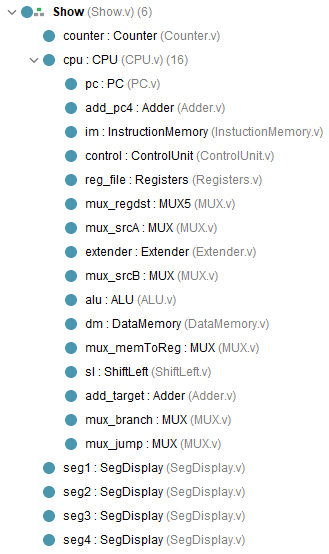
\includegraphics[width=0.4\linewidth]{fig/code_hierachy.PNG}
\caption{代码层次结构}
\label{fig:code_hierachy}
\end{figure}